\documentclass{beamer}

\mode<presentation> {
%  \usetheme{Warsaw}
	\usetheme{Boadilla}
	\setbeamercovered{transparent}
}

%\usepackage{ucs}
\usepackage[utf8]{inputenc}
\usepackage[czech]{babel}
%\usepackage{palatino}
\usepackage{graphicx}
\usepackage{listings}

\title[BitLocker šifrování v Linuxovém prostředí]{BitLocker šifrování v Linuxovém prostředí\\\small{Diplomová práce}}
\author{Vojtěch Trefný}
\institute[FAI UTB]{Fakulta aplikované informatiky UTB}
\date{4. června 2019}

\begin{document}

\begin{frame}
\maketitle
\small
\begin{tabular}[t]{@{}r@{\hspace{3pt}}p{.32\textwidth}@{}}
\textbf{Vedoucí:} & Ing. Michal Bližňák, Ph.D. \\
\textbf{Konzultant:} & Ing. Milan Brož, Ph.D. \\
\textbf{Oponent:} & Mgr. Martin Kolman \\
\end{tabular}%
\end{frame}

%%%%%%%%%%%%%%%%%%%%%%%%%%%%%%%%%%%%%%%%%%%%%%%%%%%%%%%%%%%%%%%%%%

\section{Zadání}

\begin{frame}
	\frametitle{Motivace}
	\begin{block}{Šifrování disku}
		\begin{itemize}
			\item Jediná spolehlivá metoda ochrany dat v případě ztráty nebo krádeže přenosného zařízení.
			\item Především pro ochranu notebooků a přenosných disků.
		\end{itemize}
	\end{block}

	\begin{block}{Heterogenní prostředí}
		\begin{itemize}
			\item Neexistuje jednoduchý způsob řešení šifrování v prostředí MS Windows i GNU/Linux.
			\item Bez nástrojů třetích stran nefungují nativní řešení jednoho prostředí v druhém.
			\item Multiplatformní řešení vyžadují ruční instalaci a nejsou integrována do systému.
		\end{itemize}
	\end{block}

\end{frame}

%%%%%%%%%%%%%%%%%%%%%%%%%%%%%%%%%%%%%%%%%%%%%%%%%%%%%%%%%%%%%%%%%%

\section{Cíle}

\begin{frame}
	\frametitle{Cíl práce}
	\begin{block}{}
		\begin{itemize}
			\item Prozkoumat technologii BitLocker a možnosti její podpory v linuxovém prostředí.
			\item Vytvořit nové nebo upravit stávající nástroje pro práci s BitLocker v prostředí GNU/Linux.
			\item Integrovat řešení do stávajících nástrojů tak, aby nebyla vyžadována interakce ze strany uživatele.
			\item Ideálně by uživatel neměl poznat, že nepracuje s nativním šifrováním.
		\end{itemize}
	\end{block}

\end{frame}

\begin{frame}
	\frametitle{BitLocker}

	\begin{block}{}
		\begin{itemize}
			\item Nativní šifrování disku v prostředí Microsoft Windows.
			\item Poprvé představen ve Windows Vista.
			\item Není oficiálně standardizován, ale používá standardizované kryptografické funkce:
			
			\begin{itemize}
				\item AES-CCM pro šifrování klíčů,
				\item AES-XTS (AES-CBC) pro šifrování dat a
				\item SHA256 pro odvození klíče.
			\end{itemize}
		\end{itemize}
	\end{block}

\end{frame}

\begin{frame}
	\frametitle{Struktura BitLocker zařízení}

	\begin{block}{}
		\begin{itemize}
			\item Hlavička -- identifikace zařízení
			\item FVE metadata -- klíče
			\item NTFS hlavička -- šifrovaná hlavička pro otevřené zařízení
			\item Šifrovaná data
		\end{itemize}
	\end{block}
	
	\begin{figure}[ht!]
	\begin{center}
  	  \includegraphics[width=11cm]{img/bitlocker-schema.png}
	\end{center}
	\end{figure}

\end{frame}

%%%%%%%%%%%%%%%%%%%%%%%%%%%%%%%%%%%%%%%%%%%%%%%%%%%%%%%%%%%%%%%%%%

\section{Implementace v linuxovém prostředí}

\begin{frame}
	\frametitle{LUKS/dm-crypt}

	\begin{block}{Device mapper}
		\begin{itemize}
			\item Kernelový ovladač sloužící pro tvorbu \uv{mapovaných} blokových zařízení.
			\item Primárně slouží pro vytvoření menších blokových zařízení nad jedním diskem nebo naopak spojení více disků do jednoho zařízení.
		\end{itemize}
	\end{block}
	
	

\vspace{0.5cm}

	\begin{block}{LUKS/dm-crypt}
		\begin{itemize}
			\item Nativní technologie pro šifrování disků v linuxových systémech.
			\item Crypto target slouží pro vytvoření zařízení, které při čtení/zápisu data transparentně (de)šifruje.
			\item Ve výchozím nastavení používá pro šifrování dat AES-XTS.
		\end{itemize}
	\end{block}

\end{frame}

\begin{frame}
	\frametitle{BitLocker v Linuxu}

	\begin{block}{Device mapper}
		\begin{itemize}
			\item Device mapper potřebuje znát:
			\begin{itemize}
				\item použitou šifru (AES-XTS),
				\item inicializační vektor (číslo sektoru),
				\item klíč a
				\item umístění dat na zařízení.
			\end{itemize}
		\end{itemize}
	\end{block}
	
\begin{figure}[ht!]
	\begin{center}
  	  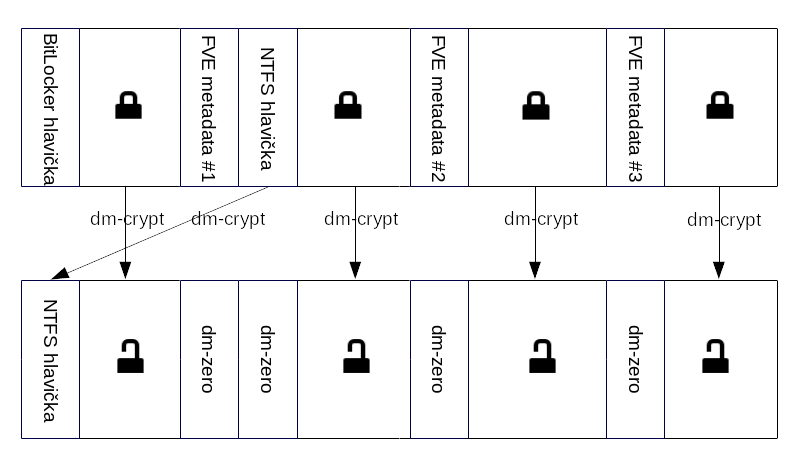
\includegraphics[width=9cm]{img/bitlocker-dm-schema.png}
	\end{center}
	\end{figure}

\end{frame}

\begin{frame}[fragile]
	\frametitle{Nástroj bitlockersetup}

	\begin{block}{}
		\begin{itemize}
			\item Nově vytvořený nástroj pro práci s BitLocker zařízeními.
			\item Umožňuje odemknout a uzamknout dané zařízení.
			\item Při odemykání:
			\begin{itemize}
				\item Z BitLocker metadat získá klíč (dešifruje jej pomocí uživatelem zadaného hesla) a strukturu zařízení (umístění jednotlivých datových oblastí) a
				\item pomocí nástroje \texttt{dmsetup} vytvoří otevřené zařízení.
			\end{itemize}
		\end{itemize}
	\end{block}

\vspace{0.5cm}
	
\begin{lstlisting}[frame=none, basicstyle=\ttfamily\small, columns=fullflexible, keepspaces=true]
$ sudo bitlockersetup open /dev/sdb1
Password for '/dev/sdb1': 
Created device mapper device '/dev/mapper/bitlocker-1f8bf...8f40'.
\end{lstlisting}

\end{frame}

\begin{frame}
	\frametitle{Integrace do existujících nástrojů}

	\begin{block}{UDisks}
		\begin{itemize}
			\item UDisks je systémový démon, který poskytuje API pro práci s blokovými zařízeními.
			\item Poskytuje také funkcionalitu pro odemykání šifrovaných zařízení.
			\item V rámci práce byla to UDisks přidána podpora pro práci s BitLocker zařízeními pomocí nástroje bitlockersetup.
			\item UDisks díky tomu označí BitLocker zařízení jako šifrovaná a poskytne funkce pro jeho odemčení a uzamčení.
			\item Z pohledu uživatelů UDisks API není rozdíl mezi zařízením šifrovaným pomocí BitLocker a LUKS/dm-crypt.
		\end{itemize}
	\end{block}
\end{frame}

\begin{frame}[fragile]
	\frametitle{Integrace do existujících nástrojů}

	\begin{lstlisting}[frame=none, escapechar=$, basicstyle=\ttfamily\small, columns=fullflexible, keepspaces=true]
/org/freedesktop/UDisks2/block_devices/sda2:
  org.freedesktop.UDisks2.Block:
...
    Id:
    IdLabel:
    $\textcolor{blue}{IdType:}$                     $\textcolor{blue}{BitLocker}$
    $\textcolor{red}{IdUUID:}$                     $\textcolor{red}{1f8bf933-8323-4c97-...}$
    $\textcolor{blue}{IdUsage:}$                    $\textcolor{blue}{crypto}$
  $\textcolor{red}{org.freedesktop.UDisks2.Encrypted:}$
    ChildConfiguration:         []
    CleartextDevice:            '/'
    $\textcolor{red}{HintEncryptionType:}$          $\textcolor{red}{BitLocker}$
\end{lstlisting}

\begin{block}{UDisks}
	\begin{itemize}
		\item Používá bitlockersetup pro identifkace BitLocker zařízení a zjištění dodatečných informací.
		\item Nabízí funkce \texttt{Unlock} a \texttt{Lock} pro odemčení a uzamření zařízení.
	\end{itemize}
\end{block}

\end{frame}

\begin{frame}
	\frametitle{Grafické rozhraní}

\begin{figure}[ht!]
	\begin{center}
  	  \includegraphics[width=11cm]{img/bitlocker-xfce.png}
	\end{center}
	\end{figure}
\end{frame}

%%%%%%%%%%%%%%%%%%%%%%%%%%%%%%%%%%%%%%%%%%%%%%%%%%%%%%%%%%%%%%%%%%

\section{Rozšíření do budoucna}

\begin{frame}
  \frametitle{Možná rozšíření do budoucna}
	\begin{block}{}
		\begin{itemize}
			\item Podpora ostatních (starších a méně obvyklých) variant BitLockeru. (Bude vyžadovat změny v kernelu.)
			\item Přidání vytvořeného nástroje do oficiálních repozitářů vybraných linuxových distribucí.
			\item Začlenění do projektu cryptsetup, který poskytuje knihovnu a nástroj pro práci s šifrovanými zařízeními v Linuxu (LUKS, VeraCrypt, Loop-AES).
		\end{itemize}
	\end{block}

\end{frame}


%%%%%%%%%%%%%%%%%%%%%%%%%%%%%%%%%%%%%%%%%%%%%%%%%%%%%%%%%%%%%%%%%%

\section{Závěr}

\begin{frame}
  \frametitle{Dotazy k obhajobě}
	\begin{block}{Otázka}
		Myslím si, že po začlenění podpory pro Bitlocker do linuxových distribucí by tato technologie
mohla sloužit jako dobrý nástroj pro přenos šifrovaných dat mezi Windows a Linuxem bez nutnosti doinstalování softwaru třetích stran. Pro plné využití tohoto potenciálu by se však hodila možnost vytvářet nová Bitlocker zařízení nejen na Windows, ale i na Linuxu. Je tvorba nových Bitlocker zařízení na Linuxu v budoucnu proveditelná?
	\end{block}
	
		\begin{block}{Odpověď}
		Teoreticky to možné je. Bohužel v BitLocker metadatech je stále mnoho neznámých položek, takže by mohlo být složité vytvořit zařízení, které bude v MS Windows skutečně stoprocentně funkční. Nabízí se také otázka, jak by se k takové implementaci postavila společnost Microsoft.
	\end{block}

\end{frame}

\begin{frame}
	\frametitle{Závěr}

	\begin{center}
	Děkuji vám za pozornost.
	\end{center}

\vspace{0.5cm}

	\begin{center}
	Prostor pro vaše dotazy.
	\end{center}
\end{frame}

\end{document}

